\documentclass{uc3mpracticas}

\usepackage{helvet}
\usepackage{multicol}
\renewcommand{\familydefault}{\sfdefault}
\usepackage{changepage}
\usepackage{geometry}
\usepackage{caption}
\usepackage{xcolor,colortbl}
\usepackage{makecell}
\usepackage{mathtools}

\usepackage{amsfonts}

\definecolor{Gray}{gray}{0.85}
\definecolor{LightCyan}{rgb}{0.88,1,1}
\definecolor{LightGreen}{rgb}{0.29,1,0.39}

\newcolumntype{g}{>{\columncolor{Gray}}l}
\newcolumntype{b}{>{\columncolor{LightCyan}}c}


%%%%%%%%%%%%%%%%%%%%%%%%%%%%%%%%%%%%%%%%%%%%%%%%%%%%%%%%%%%%%%%%%%%%%%%%%%%%%%%%
%%%                   Plantilla Prácticas UC3M                               %%%
%%%                Universidad Carlos III de Madrid                          %%%
%%%                   Alejandro Valverde Mahou                               %%%
%%%%%%%%%%%%%%%%%%%%%%%%%%%%%%%%%%%%%%%%%%%%%%%%%%%%%%%%%%%%%%%%%%%%%%%%%%%%%%%%

%Permitir cabeceras y pie de páginas personalizados
\pagestyle{fancy}

%Path por defecto de las imágenes
\graphicspath{ {./images/} }

%Declarar formato de encabezado y pie de página de las páginas del documento
\fancypagestyle{doc}{
  %Cabecera
  \headerpr[1]{Test de Primalidad - AKS}{}{Teoría Avanzada de la Computación}
  %Pie de Página
  \footerpr{}{\textbf{UC3M}}{{\thepage} de \pageref{LastPage}}
}

%Declarar formato de encabezado y pie del título e indice
\fancypagestyle{titu}{%
  %Cabecera
  \headerpr{}{}{}
  %Pie de Página
  \footerpr{}{}{}
}


\appto\frontmatter{\pagestyle{titu}}
\appto\mainmatter{\pagestyle{doc}}


\begin{document}
  %Comienzo formato título
  \frontmatter


  %Portada 1 (Centrado todo)
  \centeredtitle{Images/LogoUC3M.png}{Grado en Ingeniería Informática}{Curso 2020/2021}{Teoría Avanzada de la Computación}{Test de Primalidad}{\textit{AKS}}

  \vspace{55mm}

  \authors{Iván Miguelez García}{100383387}{Alba Reinders Sánchez}{100383444}{Alejandro Valverde Mahou}{100383383}{}{}

  \newpage

  %Índice
  \tableofcontents

\newpage

  %Comienzo formato documento general
  \mainmatter

  \begin{abstract}
    En este trabajo se realiza un estudio del algoritmo de test de primalidad \textit{AKS} desde una perspectiva analítica y empírica. Se plantea hacer el estudio dividiendo en distintas partes el algoritmo para calcular el coste computacional de cada parte.

    \vspace{2mm}

    El estudio se hará sobre el código proporcionado en la práctica, que se encuentra en el lenguaje de programación \textit{Java}. Además, se propone una traducción a \textit{Python}, para facilitar su comprensión.

  \end{abstract}



  \newpage

  \section{Introducción}

  Para estudiar la complejidad computacional del algoritmo \textit{AKS} se ha dividido el estudio en 3 hitos diferentes: \textit{Heurísticas iniciales}, \textit{cálculo del Totient} y \textit{análisis de la condición suficiente}.

  \vspace{2mm}

  El documento se divide en 3 secciones principales, una para cada hito que se ha realizado. De cada hito se realiza el análisis analítico y empírico de la parte correspondiente en el código de \textit{AKS} que se proporciona.

  \vspace{2mm}

  Para los cálculos empíricos se propone realizar cada uno de los experimentos 10 veces, obtener los tiempos de ejecución y calcular la media de dichos tiempos con el objetivo de minimizar el posible ruido que se genera al ejecutar especialmente en una máquina \textit{Windows}.


  \section{Hito 1: Heurísticas iniciales}

  Para esta primera parte de la práctica se pide realizar un estudio analítico y empírico de las dos primeras heurísticas del algoritmo \textit{AKS}, utilizado para determinar la primalidad de un número natural.

  \vspace{2mm}




  \subsection{Potencia perfecta}

  La primera heurística consiste en comprobar si un número es una potencia perfecta. Para ello, se debe cumplir la siguiente propiedad.

  $$ a^b = n \; | \; a, b \in \mathbb{N}, \; b>1$$

  Si esta propiedad se cumple, se puede afirmar que $n$ no es un número primo.


  \subsubsection{Estudio analítico}
  Se pretende determinar la complejidad temporal de los pasos del algoritmo en los que se lleva a cabo esta primera tarea. A continuación, se realiza el estudio analítico para averiguar \textit{T(n)} y \textit{O(n)}.

  \vspace{2mm}

  Para ello se tiene que analizar la estructura del código. Se puede ver que está compuesto por dos bucles \textit{do while}. El bucle exterior itera sobre $a$ y el bucle interior itera sobre $b$.

  \vspace{2mm}

  Para el análisis del bucle exterior, es necesario determinar el valor máximo de $a$.
  Se puede afirmar que, dado que el valor mínimo de $b$ es 2, el valor máximo de $a$ será $\sqrt{n}$, porque:

  $$ a^2 = n \; \Rightarrow \; a = \sqrt{n} $$

  El bucle interior requiere un desarrollo un poco mayor. Para conseguir el número de iteraciones es necesario despejarlo en la ecuación.

  \vspace{2mm}

  $$ a^{\frac{\log n}{\log a} - 1 + k} > n \Rightarrow \log a^{\frac{\log n}{\log a} - 1 + k} > \log n \Rightarrow (\frac{\log n}{\log a} - 1 + k) * \log a > \log n \Rightarrow  \frac{\log n}{\log a} - 1 + k > \frac{\log n}{\log a}$$

  $$ -1 + k > 0 \Rightarrow k > 1 $$

  Por tanto, el número de ciclos del bucle interior será 3 (Tiene que recorrer $k=0$, $k=1$ y $k=2$)

  \vspace{2mm}

  Si se unen ambas complejidades, se puede ver que para esta primera heurística, la complejidad temporal es:

  $$ T(n) = \displaystyle 3*\sqrt{n}$$

  Y el coste computacional es:

  $$ O(n) = \sqrt{n}$$


  \subsubsection{Estudio empírico}\label{empirico}

  Para realizar el estudio empírico de la comprobación de la potencia perfecta, se ha utilizado una función para generar números primos de \textit{n} dígitos. En este caso, se han generado 500 números de 5 a 9 cifras, 100 números por cada cifra, para llevar a cabo la experimentación.

  \vspace{3mm}


  Como se puede ver en la Figura \ref{fig:h1}, los tiempos obtenidos coinciden con la complejidad esperada. La complejidad de la heurística es $ O(n) = \sqrt{n} $, y haciendo uso de un optimizador de parámetros, se obtiene una curva con valor:

  $$ 1.7654419^{-07} * \sqrt{n} $$

  % \begin{itemize}
  %   \item Puede ser que no se hayan probado con números suficientemente grandes como para apreciar la curva esperada.
  %   \item Puede que el resultado esperado no esté escalado correctamente, y por tanto los valores no coincidan.
  %   \item Debido a que se ha ejecutado un código en \textit{Java} en una máquina \textit{Windows}, puede que los tiempos no estén bien medidos y tengan mucho ruido,
  % \end{itemize}
  %
  % Para próximos hitos se volverá a probar, pero con una cantidad de números mayor.

  \begin{figure}[!h]
    \centering
    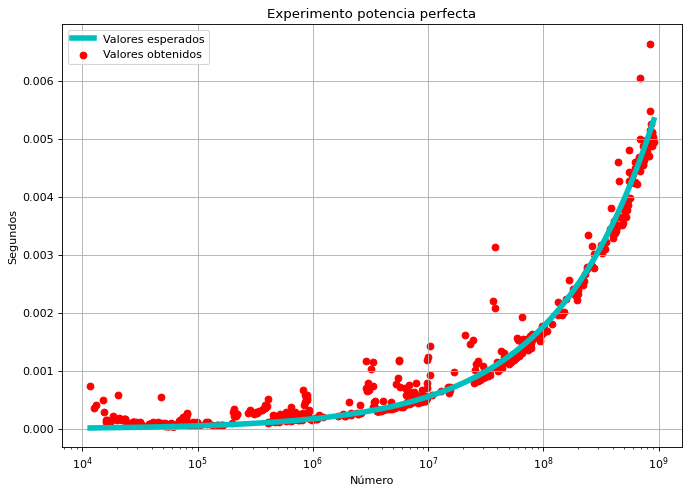
\includegraphics[width=.8\linewidth]{./Images/h1.png}
    \caption{Gráfica de tiempo del experimento potencia perfecta}
    \label{fig:h1}
  \end{figure}

  Aún así se observa cierto ruido por realizar la ejecución en \textit{Windows}, ya que se producen a la vez otros procesos ajenos que pueden influenciar en los tiempos del estudio y por tanto generar en la gráfica puntos que no se ajustan a la complejidad calculada.




  \subsection{Cálculo de \textit{r} y \textit{mcd}}

  Esta segunda heurística consiste en comprobar si se cumple la siguiente premisa:

  $$ \exists a \leq r \mid 1 < mcd(n,a) < n $$

  Si se cumple, se dice que $n$ es un número compuesto.


  \subsubsection{Estudio analítico}
  Para determinar la complejidad temporal de esta segunda tarea se tiene que dividir el estudio en dos partes. En primer lugar, se debe calcular $r$ y después calcular el $mcd$.

  \vspace{11mm}

  \textbf{Cálculo de \textit{r}}

  \vspace{2mm}


  Analizando la estructura del código, se ve que está compuesto por un bucle \textit{do while} que itera sobre $r$ y que dentro se llama a la función \textit{multiplicativeOrder()}. Esta función tiene a su vez un bucle \textit{do while} que itera sobre $k$.

  \vspace{2mm}

  Se busca el mínimo $r$ tal que:

  $$ O_r(n) > \log_2^2(n) $$

  Donde $O_r(n)$ es el orden de $n$ módulo $r$ y representa el menor $k$ tal que:

  $$ O_r(n) = k \; \Leftrightarrow \; n^k \equiv 1\pmod{r}$$


  Se sabe cuál es el máximo $r$ por el lema 4.3 de \textit{Primes is in P}\cite{primesinp}:

  $$ r \leq \lceil \log^5(n) \rceil $$

  Por lo tanto se concluye que la complejidad temporal del cálculo de $r$ es la unión de las complejidades de ambos bucles:

  $$ T(n) = \log^5(n) * \log^2(n) = \log^7(n) = O(n)$$

  \vspace{2mm}

  \textbf{Cálculo del \textit{mcd}}

  \vspace{2mm}

  Por último, para la complejidad de calcular el máximo común divisor de dos número $a$ y $b$, se tiene en cuenta el peor de los casos: cuando $a$ y $b$ son números consecutivos en la sucesión de \textit{Fibonacci}.

  \vspace{2mm}

  En este caso, el número de iteraciones del bucle es el índice del término de la sucesión, el cual se saca con la fórmula de E.Lucas:

  $$ f_n =\frac{\phi^n - (1-\phi)^n}{\sqrt{5}} $$

  cuya complejidad es $\log(n) $ porque es un cálculo directo que no hace uso de bucles.

  \vspace{2mm}


  Por tanto, la complejidad total del $mcd$:

  $$ T(n) = \log(n) * \log^5(n) = \log^6(n) = O(n)$$

  y la fórmula de la complejidad total de la heurística 2 es de:

  $$ T(n) = \log^7(n) + \log^6(n)$$

  $$ O(n) = \log^7(n)$$




  \subsubsection{Estudio empírico}

  Para esta experimentación se utilizan los mismos números que para el estudio empírico anterior. En este caso, tal como se puede ver en la Figura \ref{fig:h2}, la diferencia entre el tiempo propuesto en el estudio analítico y el empírico es algo mayor. Esto puede indicar que los cálculos del estudio analítico no sean correctos, aunque lo más probable es que se deba a la codificación del propio algoritmo de \textit{AKS}.

  \vspace{2mm}

  Resaltar que para realizar el estudio empírico, la entrada que recibe la función \textit{Totient} no es el resultado de calcular \textit{r} a partir del conjunto de números, pues los tiempos de ejecución son demasiado pequeños para poder observar un cambio significativo. Por ello, se utilizan directamente los números del conjunto con los que se obtienen tiempos de ejecución algo mayores que permiten visualizar la complejidad del algoritmo en la gráfica.


  \begin{figure}[!h]
    \centering
    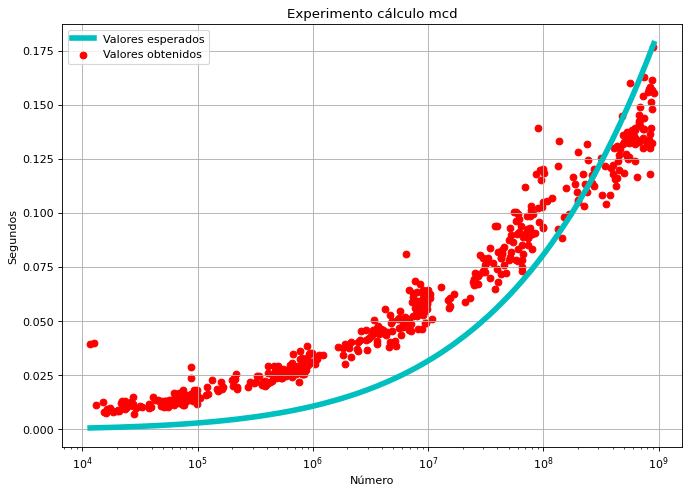
\includegraphics[width=.8\linewidth]{./Images/mcd.png}
    \caption{Gráfica de tiempo del experimento del cálculo del \textit{mcd}}
    \label{fig:h2}
  \end{figure}

  \newpage

  \section{Hito 2: Cálculo del Totient}

  En esta segunda parte, se pide realizar el estudio analítico y empírico del cálculo del \textit{Totient} ($\phi(r)$), donde $\phi(r)$ es el número de enteros positivos más pequeños o iguales que $r$ tales que $r$ es coprimo con ellos, es decir, su $mcd$ es 1.



  \subsection{Estudio analítico}

  A continuación, se realiza el estudio analítico para averiguar la complejidad temporal del algoritmo. Analizando el código se ve que la función del cálculo del \textit{Totient} está formada por un bucle \textit{for} externo y un bucle \textit{while} interno.

  \vspace{2mm}

  El bucle exterior se ejecuta como mucho $\sqrt{r}$ veces, dado que en este caso, la peor situación se da cuando $r$ es un número primo, y por tanto el bucle exterior tiene que recorrer desde $i = 2$ hasta $i = \lfloor \sqrt{n} \rfloor + 1$. Simplificando, se encuentra en $\sqrt{r}$ veces.

  \vspace{2mm}

  El bucle interno se ejecuta como mucho $\log{r}$ veces, porque el peor caso resulta cuando $ r = i^k $ donde $ k $ es un número entero e $ i $ representa el iterador del bucle. Despejando, $k = \log_ir$, y $k$ representa el número de veces que se realiza el bucle.

  \vspace{2mm}

  Para que se cumpla el peor de los casos del bucle \textit{for} exterior, $r$ tiene que ser un número primo, y por tanto el bucle \textit{while} interior no se realizará ninguna vez. En el caso de que $r$ sea el número primo, también se obtiene el valor máximo de $\phi(r)$, que es $r-1$.

  \vspace{2mm}

  La complejidad temporal de este apartado es por tanto:

  $$ T(r) = \sqrt{r-1} * \log r $$

  \vspace{5mm}

  y dado que la complejidad de $r$ es $\log^5(n)$, la complejidad es:

  $$ O(r) = \sqrt{r} * \log r $$

  $$ O(n) = \sqrt{\log^5(n)} * \log (\log^5(n)) $$



  \subsection{Estudio empírico}

  Para realizar la experimentación del cálculo del \textit{Totient} se utiliza de nuevo el mismo conjunto de números que se utilizan en el Hito 1. Observando la gráfica de la Figura \ref{fig:totient}, se ve claramente como la línea azul que representa la función de la complejidad calculada en el estudio analítico encaja con la nube de puntos rojos que representan el tiempo de ejecución medido durante la experimentación.


  \begin{figure}[!h]
    \centering
    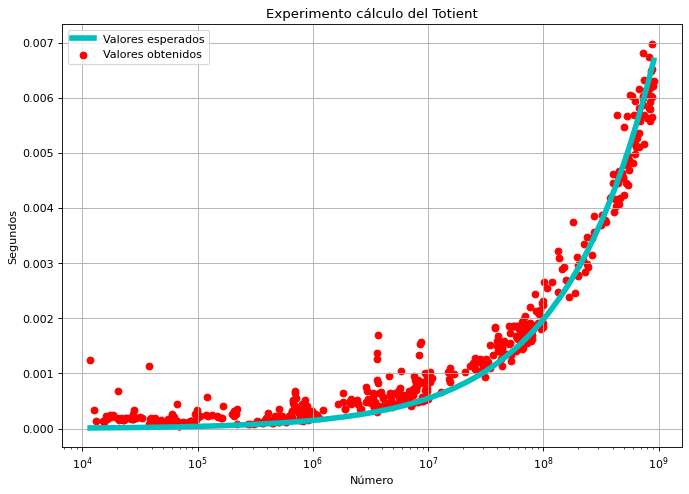
\includegraphics[width=.8\linewidth]{./Images/totient.png}
    \caption{Gráfica de tiempo del experimento cálculo del \textit{Totient}}
    \label{fig:totient}
  \end{figure}




  \section{Hito 3: Análisis de la condición suficiente}

  En esta última parte, se va a realizar el estudio empírico y analítico de la condición suficiente del algoritmo \textit{AKS}. El objetivo de esta condición es determinar la primalidad de un número. Gracias al cálculo de \textit{r}, se puede implementar una mejora en el cálculo del \textit{mcd}:

  \vspace{3mm}

  Cálculo del \textit{mcd}:

  $$ (x + a)^n \equiv (x^n + a)\pmod{n}$$


  Mejora:

  $$ (x + a)^n \equiv (x^n + a)\pmod{X^r-1}$$

  \vspace{2mm}

  La sección del código encargada de determinar la condición suficiente consta de un bucle definido por el rango que comprende la mejora implementada.




  \subsection{Estudio analítico}

  El estudio analítico de la condición suficiente de \textit{AKS} tan sólo se centra en el cálculo de la complejidad del bucle. Teniendo en cuenta la mejora anterior, el rango de número enteros que deben probarse es $[1, 2\sqrt{r}\log_2{n})$. Calculando el \textit{Totient} de \textit{r}, este rango pasa a ser $[1, 2\sqrt{\phi(r)}\log_2{n})$, disminuyendo así el número de iteraciones que la función encargada de determinar si un número es compuesto o no debe realizar. La implementación que se encuentra en la práctica difiere ligeramente con estos valores y utiliza como límite superior $\sqrt{\phi{(r)}}\log n$.

  \vspace{3mm}

  La complejidad es por tanto:

  $$ O(r) = \sqrt{\phi{(r)}} * \log n $$


  \subsection{Estudio empírico}

  Para realizar el estudio empírico, inicialmente se utilizaron los mismos números que se usaron en los hitos anteriores. Sin embargo, a partir de las 5 cifras el tiempo necesario para calcular la condición suficiente de un número era demasiado elevada para realizar pruebas. Por lo tanto, se creó un generador de números primos y se seleccionaron 100 números de 3 cifras y 100 números de 4 cifras. El resultado es un conjunto de 200 números.

  \vspace{3mm}

  Analizando la Figura \ref{fig:suficiente}, la línea continua que representa la función de la complejidad de la condición suficiente, no encaja con la nube de puntos que representa los tiempos de ejecución obtenidos durante la experimentación. Esto se debe a que no se tiene en cuenta la complejidad de las funciones que pertenecen a la librería \textit{Poly}.

  \begin{figure}[!h]
    \centering
    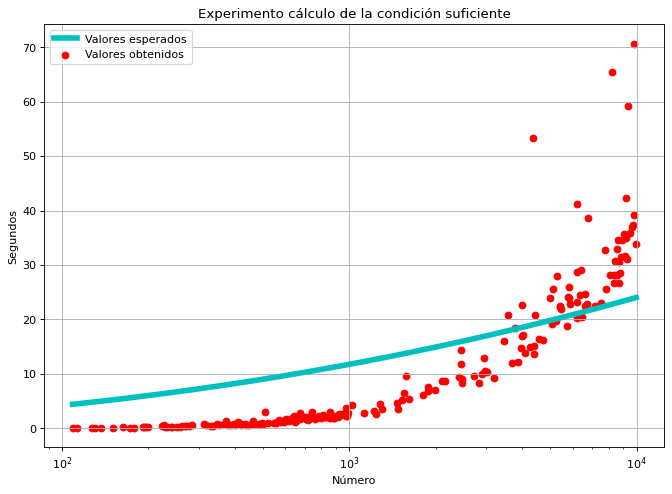
\includegraphics[width=.8\linewidth]{./Images/suficiente.png}
    \caption{Gráfica de tiempo del experimento cálculo de la condición suficiente respecto a \textit{limit}}
    \label{fig:suficiente}
  \end{figure}

  Según la documentación oficial \textit{Primes in P}\cite{primesinp}, la complejidad computacional de este apartado es:

  $$ O(\log^\frac{21}{2}n) $$

  \vspace{2mm}

  Al comparar esta complejidad con los resultados empíricos, se observa en la Figura \ref{fig:suficiente2} como la función se ajusta adecuadamente a la nube de puntos, concluyendo así el estudio empírico.

  \begin{figure}[!h]
    \centering
    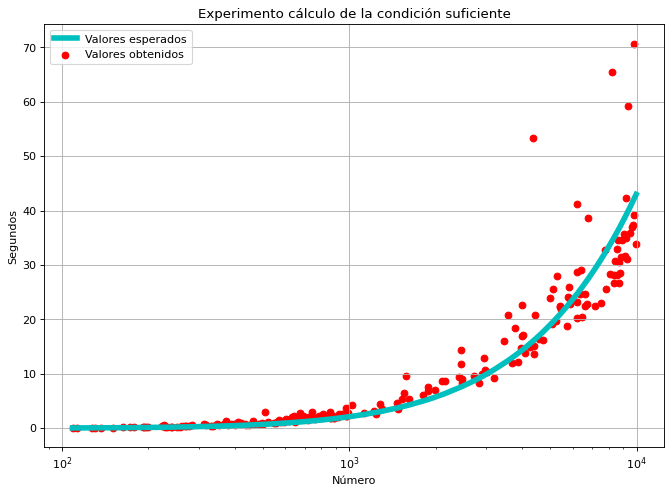
\includegraphics[width=.8\linewidth]{./Images/suficiente2.png}
    \caption{Gráfica de tiempo del experimento cálculo de la condición suficiente respecto a la complejidad descrita en el \textit{paper} original\cite{primesinp}}
    \label{fig:suficiente2}
  \end{figure}



  \newpage

  \section{Conclusiones}

  Dado que la complejidad más alta es la que pertenece al Hito 3, predomina sobre el resto de complejidades, y se puede afirmar, tal y como se menciona en el \textit{paper} original\cite{primesinp}, que la complejidad del algoritmo de test de primalidad \textit{AKS} es $ O(\log^\frac{21}{2}n) $. Los resultados teóricos se aproximan con bastante precisión a los resultados empíricos, confirmando que la implementación estudiada durante la práctica comparte una complejidad similar con la teoría.

  \vspace{3mm}

  Inicialmente se propuso realizar una traducción a \textit{Python} del código original para facilitar su comprensión. Esta implementación se llevó a cabo hasta la función \textit{Totient}. Además, se realizó una investigación previa a la traducción y se encontró un proyecto\cite{aks_git} que propone ciertas mejoras a la hora de codificar el algoritmo.

  \newpage

  \bibliographystyle{unsrt}
  \bibliography{bibliography}



\end{document}
